\documentclass{article}

\usepackage[main=english,vietnamese]{babel}
\usepackage[T1]{fontenc}
\usepackage[utf8]{inputenc}
\usepackage[sexy]{evan}
\usepackage{matchsticks}
\usepackage{wrapfig}
\usepackage{listings}

\newtheorem{hint}{Hint}

\title{A straight line is the shortest distance between two points}
\author{Nghia Doan}
\date{\today}

\begin{document}

\maketitle

In this article, we explore some basic properties of broken lines.

\begin{fact*}[Triangle Inequality]
    \label{fact:triangle-inequality}
    For any three points $A,B,C$, \[ AB + BC \ge AC, \]
    The equality holds if and only if $A, B,$ and $C$ are collinear.
\end{fact*}

\begin{fact*}[Broken Line Inequality]
    \label{fact:broken-line-inequality}
    For any points $A_1,A_2,\ldots,A_n$, $A_1A_2 + A_2A_3 + \ldots + A_{n-1} A_{n} \ge A_1 A_n.$
    The equality holds if and only if $A_1,A_2,\ldots,A_{n-1},$ and $A_n$ are collinear.
\end{fact*}

\begin{lemma*}[Heron's Problem]
    \label{lemma:heron-problem}
    Two points $A$ and $B$ lie on one side of a straight line $l$.
    $C$ is a point on on $l$.
    The sum $CA+CB$ is minimal if and only if $C = BC' \cap \ell$, where $B'$ is the reflection of $B$ over $l$. 
\end{lemma*}

\begin{center}
    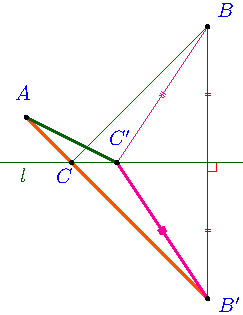
\includegraphics[width=4cm]{./asy/pdf/heron-problem-1.pdf}
\end{center}

\newpage

\begin{example*}[Cross-section of a cube]

    Lilian cuts a cube with side length $1.$ She got a with a hexagon cross-section as shown below.
    What is the minimal value of the hexagon perimeter $AB+BC+CD+DE+EF+FA$?
\end{example*}

\begin{center}
    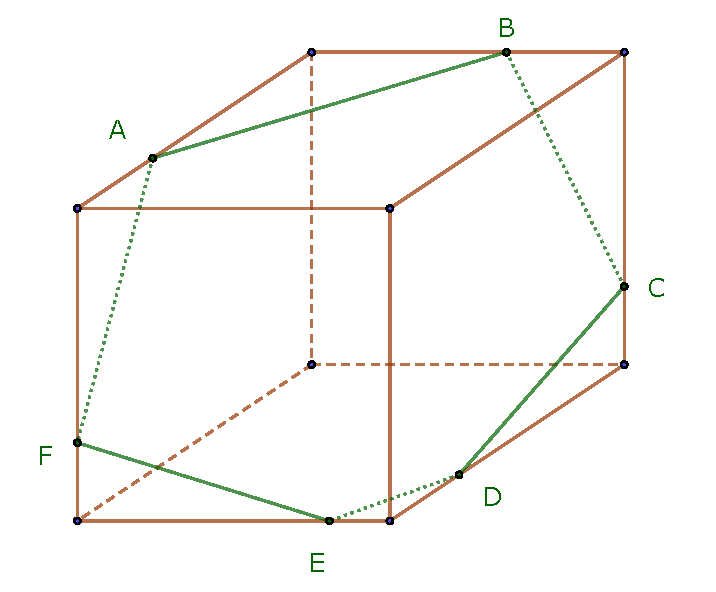
\includegraphics[width=6.5cm]{./svg/pdf/pi-2023-02-01.pdf}
\end{center}

\begin{soln}
    The diagram below is obtained by unfolding the cube into a net. The hexagon perimeter forms a broken line $ABCDEFA'.$
    \begin{center}
        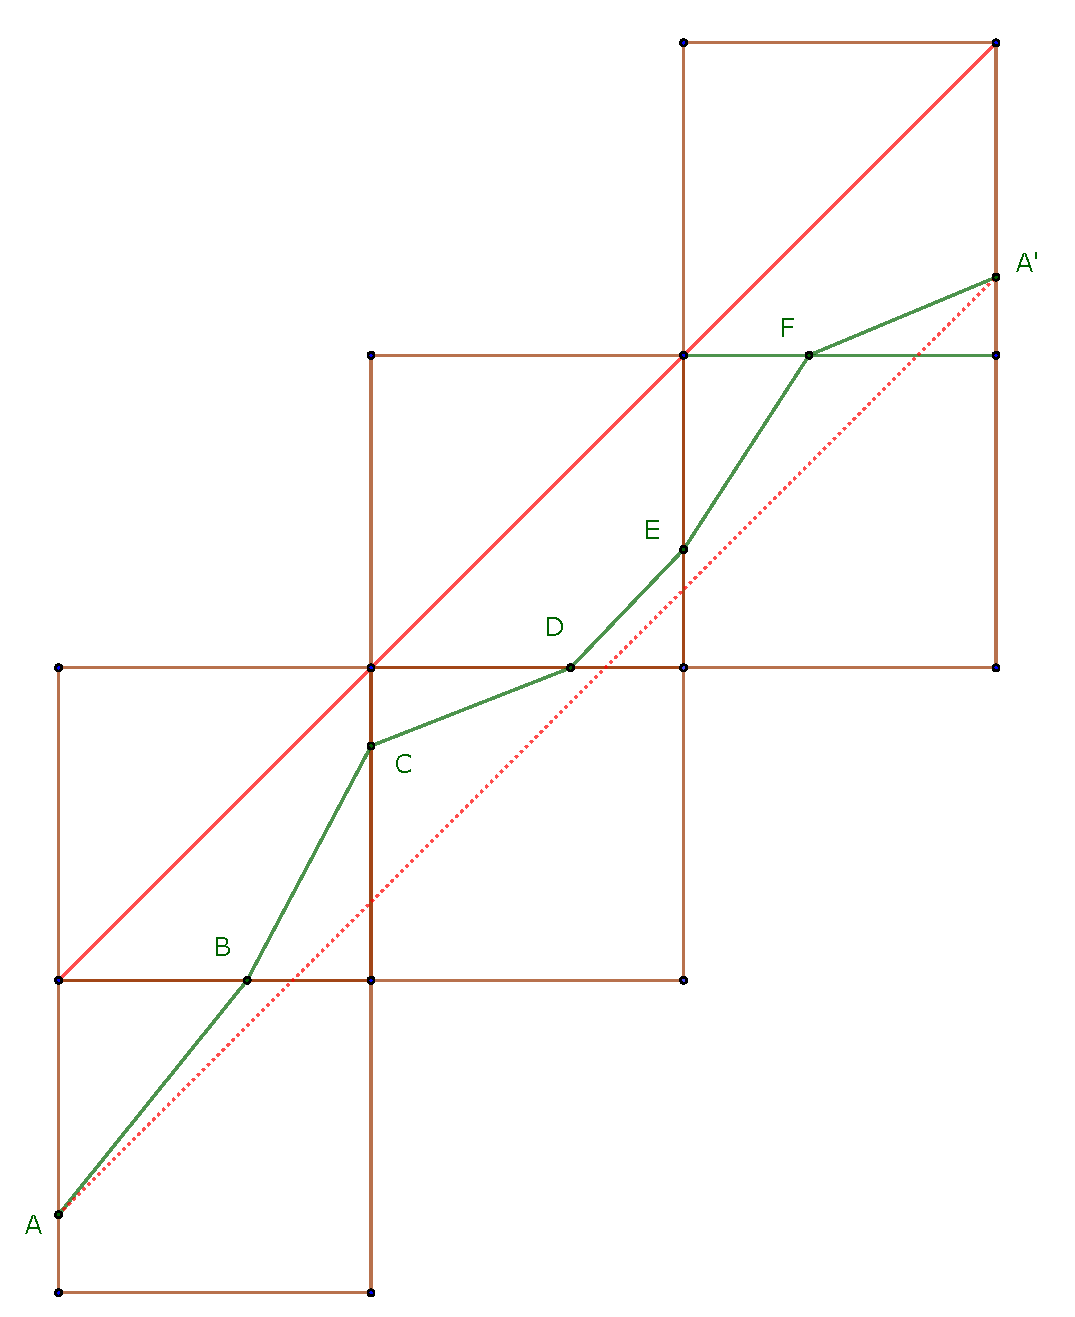
\includegraphics[width=9.5cm]{./svg/pdf/pi-2023-02-02.pdf}
    \end{center}    
    This is always larger or equal the distance $AA',$ which is same as three times the diagonal of the unit square.
    Hence the perimeter is always at least $\boxed{3\sqrt{2}}.$
\end{soln}

\begin{example*}[Diagonal of a hexagon]

    $ABCDEF$ is a convex hexagon, where $\angle A \ge 90\dg$ and $\angle D \ge 90\dg.$
    Prove that $BC+CE+EF+FB\ge 2AD.$
\end{example*}

\begin{center}
    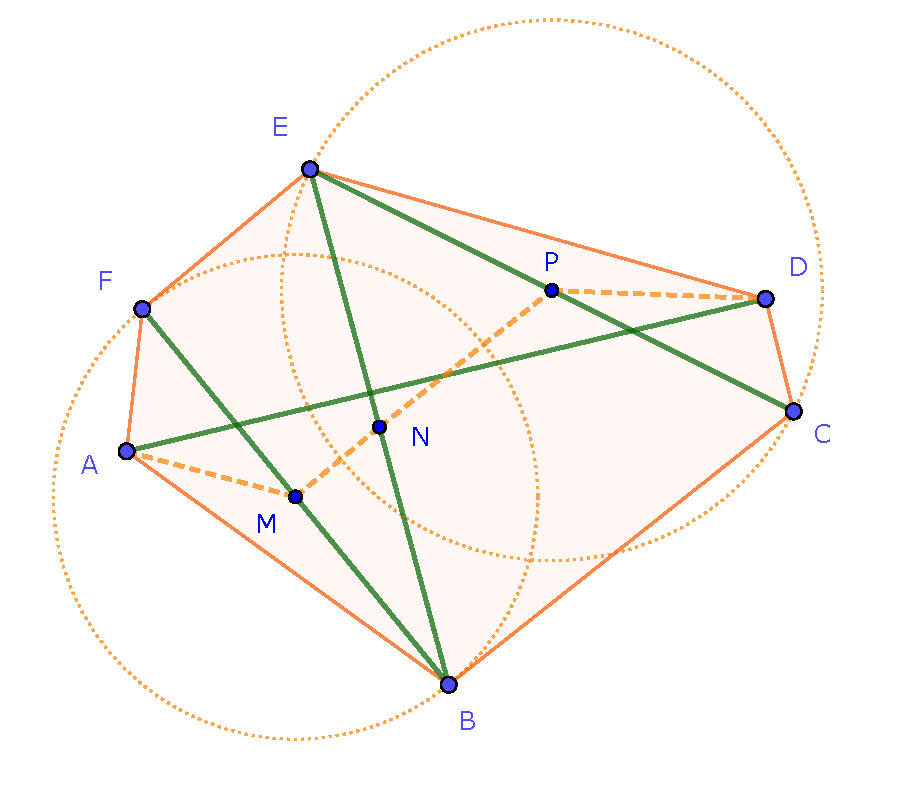
\includegraphics[width=10.5cm]{./svg/pdf/pi-2023-02-03.pdf}
\end{center}

\begin{proof}
    Let $M, N,$ and $P$ be the midpoints of $BF, BE,$ and $CE,$ respectively.
    Since any broken line is longer or equal the distance between two endpoints, so $AD\le AM+MN+NP+PD.$
    $MN$ is the median segment in $\triangle BEF,$ thus $FE = 2MN.$ Similarly $BC=2NP.$
    In $\triangle ABF,$ $\angle A \ge 90\dg,$ thus $BF \ge 2AM.$ Similarly $CE \ge 2DP.$
    Therefore $BC+CE+EF+FB \ge 2(AM+MN+NP+PD) = 2AD.$
\end{proof}

\newpage

\begin{example*}[Romanian Math Olympiad]
   
    Let $ABCD$ be a convex quadrilateral. It is known that the circles with diameter $AB$ and $CD$ are externally tangent,
    and so are the circles with diameters $AD$ and $BC.$
    Prove that $ABCD$ is a rhombus.
\end{example*}

\begin{center}
    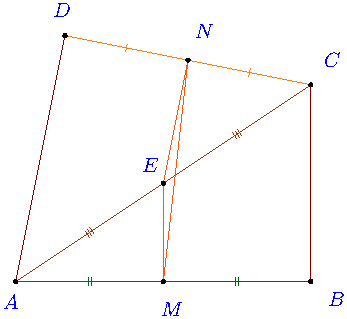
\includegraphics[width=5.5cm]{./asy/pdf/romanian-pb-gt-40.pdf}
\end{center}

\begin{proof}
    We first prove a claim.
    \begin{claim*}
        Let $M$ and $N$ be the midpoint of $AB$ and $CD$, respectively, then $AD+ BC \ge 2MN.$
    \end{claim*}

    \begin{subproof}
        Let $E$ be the midpoint of $AC.$ It is easy to see that 
        \[
            MN \le ME+EN = \frac{BC}{2} + \frac{AD}{2} = \frac{AD+BC}{2}
        \]
        The equality can happen if and only if $MN$ intersect $AC$ at the midpoint of $AC$, so $MN \parallel AD \parallel BC.$
    \end{subproof}
    By the claim $AD+BC \ge 2MN, \text{\ similarly\ } AB+CD \ge 2PQ,$ thus 
    \[ 
        AB+BC+CD+DA \ge 2(MN+PQ) \qquad (*)
    \]
   
    Now, let $P$ and $Q$ be the midpoints of $BC$ and $AD$, respectively.
    Since the circles of diameters $AB$ and $CD$ are externally tangent so $AB+CD = 2MN,$ similarly $AD+BC = 2.$
    Thus 
    \[ 
        AB+BC+CD+DA = 2(MN+PQ) \qquad (**)
    \]

    (**) implies the existence of equality in (*), so $MN \parallel AD \parallel BC$ and $PQ \parallel AB \parallel CD$.
    Thus $ABCD$ is a parallelogram, and $MN = AD = BC.$ Similarly $AB=CD.$ Since $AB +CD = 2MN$ (see above), therefore
    \[
        AD = BC = MN = AB = CD.
    \]

    Hence, \framebox{$ABCD$ is a rhombus.}
\end{proof}

\end{document}